% !TeX spellcheck = en_US
% !TeX encoding = UTF-8
\documentclass{beamer}

\mode<presentation> { \usetheme{Madrid} }

\usepackage{graphicx, graphics}
\usepackage[notocbib]{apacite}
\usepackage[style=iso]{datetime2}
\usepackage{enumerate}
\providecommand\thispdfpagelabel[1]{}
\DeclareGraphicsExtensions{.pdf, .png, .jpg, .gif}

\AtBeginSection[]
{
    \begin{frame}
        \vfill
        \centering
        \begin{beamercolorbox}[sep=8pt,center,shadow=true,rounded=true]{title}
            \usebeamerfont{title}
            \thesection. \insertsectionhead
            \par
        \end{beamercolorbox}
        \vfill
    \end{frame}
}

\AtBeginSubsection[]
{
    \begin{frame}
        \vfill
        \centering
        \begin{beamercolorbox}[sep=8pt, center, shadow=true, rounded=true]{title}
            \usebeamerfont{title}
            \thesection. \insertsectionhead
            \par
        \end{beamercolorbox}
        \begin{beamercolorbox}[sep=4pt, center, shadow=true, rounded=true]{title}
            \usebeamerfont{subtitle}
            \thesection.\thesubsection. \insertsubsectionhead
            \par
        \end{beamercolorbox}
        \vfill
    \end{frame}
}

\title[PTB]{Metagenome Analysis of Preterm Birth}

\author[Jaewoong Lee]
{
    Jaewoong Lee
    \and
    Semin Lee
}

\institute[UNIST BME]
{
    Department of Biomedical Engineering
    \newline
    Ulsan National Institute of Science and Technology
    \medskip
    \newline
    \textit{jwlee230@unist.ac.kr}
}

\date{\today}

\begin{document}
    \begin{frame}
        \titlepage
    \end{frame}

	\begin{frame}
        \frametitle{Overview}
        \tableofcontents[hideallsubsections]
    \end{frame}

    \section{Introduction}
    \begin{frame}
        \frametitle{Microbiome}

        \begin{itemize}
            \item Microbiota: the microorganisms which live inside \& on humans \cite{micro1}
            \item Microbiome: $10^{13}$ to $10^{14}$ microorganisms whose which collective genome \cite{micro2}
        \end{itemize}

        \begin{figure}
            \includegraphics[width=0.3 \linewidth]{figures/microbiome.jpg}
            \caption{Concept of a core human microbiome \protect \cite{micro1}}
        \end{figure}
    \end{frame}

    \begin{frame}
        \frametitle{rRNA}

        \begin{itemize}
            \item Ribosomal RNA
            \item Well-known as a key to phylogeny \cite{rrna1}
        \end{itemize}
    \end{frame}

    \begin{frame}
        \frametitle{Preterm Birth (PTB)}

        PTB:
        \begin{enumerate}
            \item PTB $<$ 37 GW (Gestational week)
            \item Normal $\ge$ 37 GW
        \end{enumerate}

        Detailed PTB:
        \begin{enumerate}
            \item Early PTB $<$ 34 GW
            \item 34 GW $\le$ Late PTB $<$ 37 GW
            \item Normal $\ge$ 37 GW
        \end{enumerate}

        \cite{premature1, premature2}
    \end{frame}

    \section{Materials}
    \begin{frame}
        \frametitle{16S rRNA Sequencing}

        \textbf{16S rRNA sequencing} is the \textit{reference method} for bacterial taxonomy \& identification \cite{16S1}

        Three main reasons \cite{16S2}:
        \begin{itemize}
            \item 16S rRNA exists in almost all bacteria
            \item Functions of the 16S rRNA has not changed over evolution.
            \item 16S rRNA is large enough for bioinformatics
        \end{itemize}
    \end{frame}

    \begin{frame}
        \frametitle{Data Composition}
        \begin{itemize}
            \item JBNU/Helixco data
            \begin{itemize}
                \item First data
                \item Second data
                \item Stool data
            \end{itemize}
        \end{itemize}

        \begin{table}
            \centering
            \caption{Sample Information}
            \begin{tabular}{c|ccc}
    Data & Participants & Samples & Remarks \\ \hline
    First & 24 & 107 & - \\
    Second & 35 & 288 & - \\
    Stool & 63 & 126 & Stool \\
    EBI & 18 & 1016 & Only Normal \\
    HMP & 1572 & 9205 & Only Premature \\
\end{tabular}

        \end{table}
    \end{frame}

    \section{Methods}
    \begin{frame}
        \frametitle{Qiime 2 Workflow}

        \begin{figure}
            \includegraphics[width=0.8 \linewidth]{figures/qiime.png}
            \caption{QIIME 2 workflow \protect\cite{qiime1, qiime2, qiime3}}
        \end{figure}
    \end{frame}

    \section{Results}
    \subsection{Data Processing with Qiime}
    \begin{frame}
        \frametitle{Filtering with Quality Score}

        Drawback between:
         \begin{itemize}
            \item Longer sequence read
            \item Higher quality value
        \end{itemize}

        $\therefore$ Select the maximum length $n$ where:
        \begin{equation}
            \begin{array}{c}
                \forall n_i \in \{ n_k | \mbox{MedianQualityScore} \geq 30 \} \\
                \exists ! n \in \{n_i\} : n \geq n_i
            \end{array}
        \end{equation}
    \end{frame}

    \begin{frame}
        \frametitle{Quality Score from JBNU/Helixco Data}

        \begin{figure}
            $\begin{array}{cc}
                \includegraphics[width=0.4 \linewidth]{figures/QualityFilter/EverythingForward.png}
                &
                \includegraphics[width=0.4 \linewidth]{figures/QualityFilter/EverythingReverse.png}
                \\
                \mbox{(a) Forward} & \mbox{(b) Reverse} \\
            \end{array}$
            \caption{Quality Score Plot}
        \end{figure}

        \begin{itemize}
            \item $\ell_{Forward} = 300$
            \item $\ell_{Reverse} = 245$
        \end{itemize}
    \end{frame}

    \begin{frame}
        \frametitle{Denoising Techinques}

        \begin{itemize}
            \item DADA2: Amplicon Sequence Variants (ASVs) \cite{DADA2}
            \item Deblur: Operational Taxonomic Units (OTUs) \cite{Deblur1}
        \end{itemize}

        \begin{figure}
            \includegraphics[width=0.4 \linewidth]{figures/tikz/denoising.pdf}
            \caption{Denoising Algorithms}
        \end{figure}
    \end{frame}

    \begin{frame}
        \frametitle{Taxonomy Classification}

        \begin{itemize}
            \item Greengenes (GG) \cite{greengenes1}
            \item SILVA \cite{silva1, silva2}
            \item Human Oral Microbiome Database (HOMD) \cite{homd1}
        \end{itemize}

        “A \textbf{higher} performance at taxonomic levels above \textit{genus level}; \\
        but performance appears to \textbf{drop} at \textit{species level}” \cite{performance1}
    \end{frame}

    \subsection{Abundance Test with ANCOM}
    \begin{frame}
        \frametitle{ANCOM}

        \begin{itemize}
            \item Analysis with composition of microbiome \cite{ANCOM1}
            \item ANCOM detects significantly abundant taxa, while maintain high statistical power
            \item Find taxa that can divide each classes
        \end{itemize}
    \end{frame}

    \begin{frame}
        \frametitle{ANCOM with Detail PTB}

        \begin{figure}
            $\begin{array}{ccc}
                \includegraphics[width=0.3 \linewidth]{figures/ANCOM/DADA2/homd/everything.DADA2.homd.Neonate-1day.pseudocount.Detail_PTB.pdf}
                &
                \includegraphics[width=0.3 \linewidth]{figures/ANCOM/DADA2/homd/everything.DADA2.homd.Neonate-3day.pseudocount.Detail_PTB.pdf}
                &
                \includegraphics[width=0.3 \linewidth]{figures/ANCOM/DADA2/homd/everything.DADA2.homd.Neonate-5day.pseudocount.Detail_PTB.pdf}
                \\
                \mbox{(a) 1-day} & \mbox{(b) 3-day } & \mbox{(c) 5-day} \\
            \end{array}$
            \caption{ANCOM for Detail PTB from Neonatal Mouth with DADA2+HOMD}
        \end{figure}
    \end{frame}

    \subsection{Abundance Test with LefSe}
    \begin{frame}
        \frametitle{LefSe}

        \begin{itemize}
            \item Linear discriminant analysis Effect Size \cite{lefse1}
            \item LefSe finds the features likely to explicate differences between groups
        \end{itemize}
    \end{frame}

    \begin{frame}
        \frametitle{LefSe with Detail PTB}

        \begin{figure}
            $\begin{array}{ccc}
                \includegraphics[width=0.3 \linewidth]{figures/LEfSe/Default/everything.Deblur.silva.Cervix.pdf}
                &
                \includegraphics[width=0.3 \linewidth]{figures/LEfSe/Default/everything.Deblur.silva.Mouth.pdf}
                &
                \includegraphics[width=0.3 \linewidth]{figures/LEfSe/Default/everything.Deblur.silva.Vagina.pdf}
                \\
                \mbox{(a) Cervix} & \mbox{(b) Maternal Mouth} & \mbox{(c) Vagina} \\
            \end{array}$
            \caption{LefSe for Detail PTB with Deblur + Silva}
        \end{figure}
    \end{frame}

    \subsection{Taxonomy Overview}
    \begin{frame}
        \frametitle{Abundance Distribution}

        \begin{figure}
            \includegraphics[width=0.8 \linewidth]{figures/Step53/everything.DADA2.homd.pdf}
            \caption{Abundance distribution}
        \end{figure}
    \end{frame}

    \begin{frame}
        \frametitle{t-SNE with Abundance}

        \begin{figure}
            $\begin{array}{cc}
                \includegraphics[width=0.4 \linewidth]{figures/tSNE/everything.DADA2.homd.uncorrected/All+Data.pdf}
                &
                \includegraphics[width=0.4 \linewidth]{figures/tSNE/everything.DADA2.homd/Mouth+Data.pdf}
                \\
                \mbox{(a) All} & \mbox{(b) Mother Mouth} \\
            \end{array}$
            \caption{t-SNE plot with Taxonomy Abundance}
        \end{figure}
    \end{frame}

    \begin{frame}
        \frametitle{Proportion Distribution}

        \begin{figure}
            \includegraphics[width=0.8 \linewidth]{figures/Step53_Proportion/everything.DADA2.homd.pdf}
            \caption{Proportion distribution}
        \end{figure}
    \end{frame}

    \begin{frame}
        \frametitle{t-SNE with Proportion}

        \begin{figure}
            $\begin{array}{cc}
                \includegraphics[width=0.4 \linewidth]{figures/tSNE_Proportion/everything.DADA2.homd.uncorrected/All+Data.pdf}
                &
                \includegraphics[width=0.4 \linewidth]{figures/tSNE_Proportion/everything.DADA2.homd/Mouth+Data.pdf}
                \\
                \mbox{(a) All} & \mbox{(b) Mother Mouth} \\
            \end{array}$
            \caption{t-SNE plot with Taxonomy Abundance}
        \end{figure}
    \end{frame}

    \subsection{Diversity Index}
    \begin{frame}
        \frametitle{Diversity Indices}

        \begin{figure}
            \includegraphics[width=0.6 \linewidth]{figures/phylogenic.jpg}
            \caption{Three dimensions of phylogenic information \protect\cite{phylogenetic1}}
        \end{figure}

        \begin{itemize}
            \item A quantitative measure that shows richness, divergence, and regularity \cite{phylogenetic1}
            \item Alpha diversity indices: the richness of taxa \textbf{at a single community}
            \item Beta diversity indices: the taxonomic differentiation \textbf{between communities}
        \end{itemize}
    \end{frame}

    \begin{frame}[allowframebreaks]
        \frametitle{Violin Plot with Alpha diversity}

        \begin{figure}
            $\begin{array}{cc}
                \includegraphics[width=0.4 \linewidth]{figures/AlphaDiversity/everything.DADA2/All+Detail_Premature+faith_pd.pdf}
                &
                \includegraphics[width=0.4 \linewidth]{figures/AlphaDiversity/everything.DADA2/Mouth+Detail_Premature+faith_pd.pdf}
                \\
                \mbox{(a) All} & \mbox{(b) Mother Mouth} \\
            \end{array}$
            \caption{Detail premature \& Faith's PD}
        \end{figure}

        \begin{figure}
            $\begin{array}{cc}
                \includegraphics[width=0.4 \linewidth]{figures/AlphaDiversity/everything.DADA2/All+Detail_Premature+observed_otus.pdf}
                &
                \includegraphics[width=0.4 \linewidth]{figures/AlphaDiversity/everything.DADA2/Mouth+Detail_Premature+observed_otus.pdf}
                \\
                \mbox{(a) All} & \mbox{(b) Mother Mouth} \\
            \end{array}$
            \caption{Detail premature \& Observed OTUs}
        \end{figure}

        \begin{figure}
            $\begin{array}{cc}
                \includegraphics[width=0.4 \linewidth]{figures/AlphaDiversity/everything.DADA2/All+Detail_Premature+pielou_e.pdf}
                &
                \includegraphics[width=0.4 \linewidth]{figures/AlphaDiversity/everything.DADA2/Mouth+Detail_Premature+pielou_e.pdf}
                \\
                \mbox{(a) All} & \mbox{(b) Mother Mouthy} \\
            \end{array}$
            \caption{Detail premature \& Pielou Evenness}
        \end{figure}

        \begin{figure}
            $\begin{array}{ccc}
                \includegraphics[width=0.4 \linewidth]{figures/AlphaDiversity/everything.DADA2/Mouth+Detail_Premature+shannon.pdf}
                &
                \includegraphics[width=0.4 \linewidth]{figures/AlphaDiversity/everything.DADA2/Neonate-3day+Detail_Premature+shannon.pdf}
                \\
                \mbox{(a) All} & \mbox{(b) Mother Mouth} \\
            \end{array}$
            \caption{Detail premature \& Shannon Entropy}
        \end{figure}

    \end{frame}

    \begin{frame}[allowframebreaks]
        \frametitle{Cluster map with Beta diversity}

        \begin{figure}
            \includegraphics[width=\linewidth]{figures/Step47/everything.DADA2.weighted_unifrac.pdf}
            \caption{Cluster map with Weighted UniFrac distance index for DADA2}
        \end{figure}

        \begin{figure}
            $\begin{array}{ccc}
                \includegraphics[width=0.3 \linewidth]{figures/Step47-2/everything.DADA2.weighted_unifrac.Sites/Mouth.pdf}
                &
                \includegraphics[width=0.3 \linewidth]{figures/Step47-2/everything.DADA2.weighted_unifrac.Sites/Neonate-3day.pdf}
                &
                \includegraphics[width=0.3 \linewidth]{figures/Step47-2/everything.DADA2.weighted_unifrac.Sites/Neonate-3day.pdf}
                \\
                \mbox{(a) Mouth } & \mbox{(b) Neonate 3-day} & \mbox{(c) Neonate 5-day} \\
            \end{array}$
            \caption{Clustermap with Site separation}
        \end{figure}
    \end{frame}

    \subsection{Taxonomy Analyses}
    \begin{frame}
        \frametitle{Volcano plot}

        \begin{figure}
            $\begin{array}{ccc}
                \includegraphics[width=0.3 \linewidth]{figures/Step44/everything.DADA2.homd/Mouth.pdf}
                &
                \includegraphics[width=0.3 \linewidth]{figures/Step44/everything.DADA2.homd/Neonate-3day.pdf}
                &
                \includegraphics[width=0.3 \linewidth]{figures/Step44/everything.DADA2.homd/Neonate-5day.pdf}
                \\
                \mbox{(a) Mouth} & \mbox{(b) Neonate 3-day} & \mbox{(c) Neonate 5-day} \\
            \end{array}$
            \caption{Deferentially expressed taxa}
        \end{figure}
    \end{frame}

    \begin{frame}
        \frametitle{Shared Taxonomy with Neonates \& Mothers}

        \begin{figure}
            \includegraphics[width=0.6 \linewidth]{figures/Step48/everything.DADA2.homd.pdf}
            \caption{Shared Taxonomy with Neonates \& Mothers}
        \end{figure}
    \end{frame}

    \begin{frame}[allowframebreaks]
        \frametitle{Correlation between Taxonomy \& Clinical data}

        \begin{figure}
            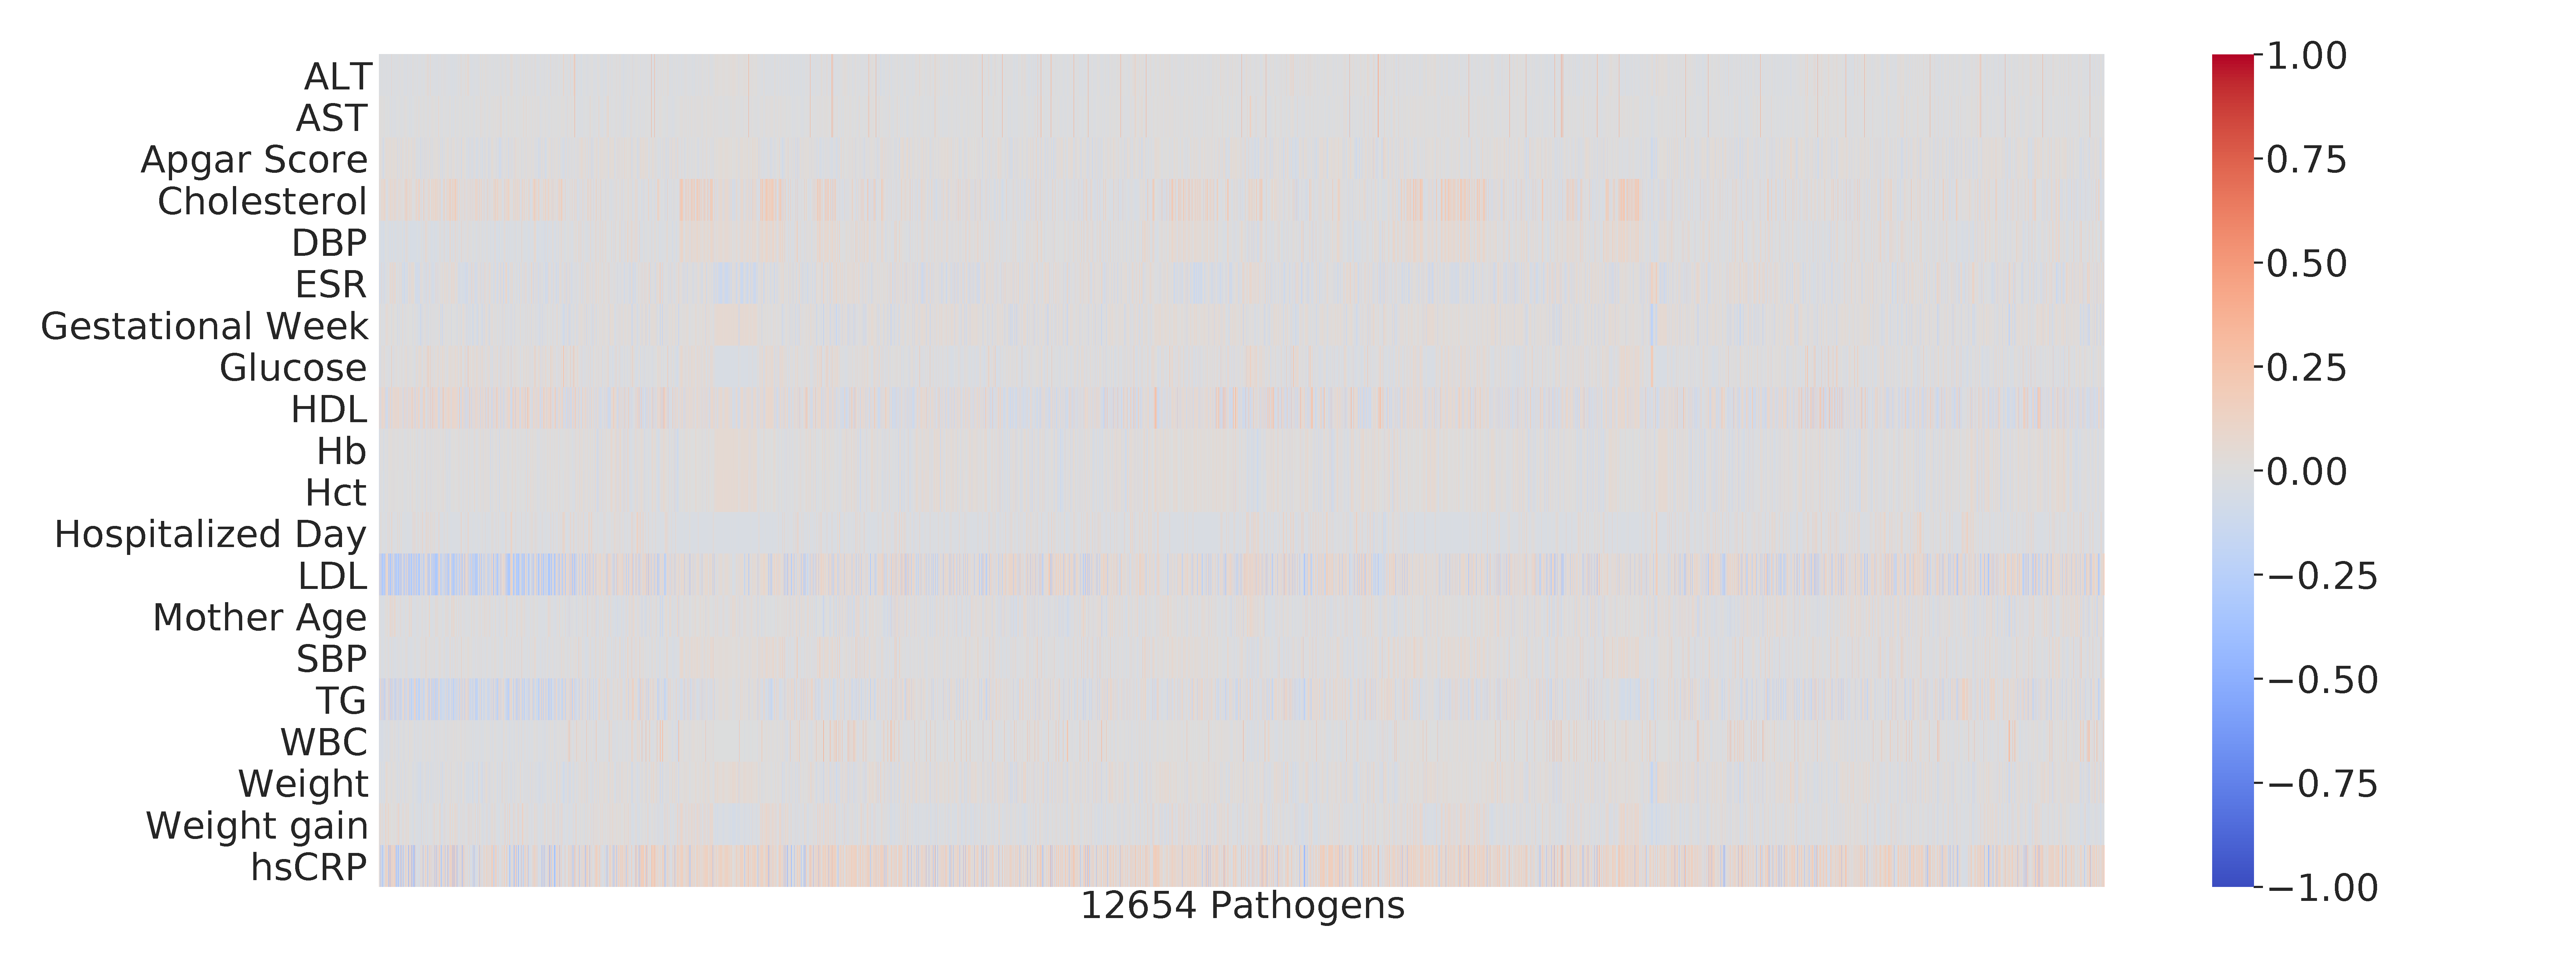
\includegraphics[width=\linewidth]{figures/Step49/DADA2/homd/everything.DADA2.homd.pearson.pdf}
            \caption{Pearson Correlation between taxonomy \& clinical Data}
        \end{figure}

        \begin{figure}
            $\begin{array}{c}
                \includegraphics[width=0.4 \linewidth]{figures/Step49-2/everything.Deblur.homd.pearson.Sites/Mouth.pdf}
                \\
                \mbox{(a) Mouth} \\

                \includegraphics[width=0.4 \linewidth]{figures/Step49-2/everything.Deblur.homd.pearson.Sites/Neonate-3day.pdf}
                \\
                \mbox{(b) Neonate 3-day} \\


                \includegraphics[width=0.4 \linewidth]{figures/Step49-2/everything.Deblur.homd.pearson.Sites/Neonate-5day.pdf}
                \\
                \mbox{(c) Neonate 5-day} \\
            \end{array}$
            \caption{Person Correlation with Site separation}
        \end{figure}
    \end{frame}

    \begin{frame}
        \frametitle{Correlation Plot}
    \end{frame}

    \subsection{Machine Learning}
    \begin{frame}
        \frametitle{ML algorithm comparison}

        \begin{figure}
            \includegraphics[width=\linewidth]{figures/ML.png}
            \caption{Classification Comparison \protect\cite{sklearn1}}
        \end{figure}
    \end{frame}

    \begin{frame}[allowframebreaks]
        \frametitle{Random Forest with (Early vs. Late vs. Full)}

        \begin{figure}
            \includegraphics[width=0.8 \linewidth]{figures/RandomForest/RF.DADA2.homd/Mouth+metrics.pdf}
            \caption{RF evaluations with feature counts}
        \end{figure}

        \begin{figure}
            \includegraphics[width=0.5 \linewidth]{figures/RandomForest/RF.DADA2.homd/Mouth+heatmap.pdf}
            \caption{RF confusion matrix}
        \end{figure}

        \begin{figure}
            \includegraphics[width=0.5 \linewidth]{figures/RandomForest/RF.DADA2.homd/Mouth+Violin_0.pdf}
            \caption{RF most important taxa}
        \end{figure}
    \end{frame}

    \begin{frame}[allowframebreaks]
        \frametitle{Random Forest with (Early vs. Late + Full)}

        \begin{figure}
            \includegraphics[width=0.8 \linewidth]{figures/RandomForest/RF-two.DADA2.homd/Mouth+metrics.pdf}
            \caption{RF evaluations with feature counts}
        \end{figure}

        \begin{figure}
            \includegraphics[width=0.5 \linewidth]{figures/RandomForest/RF-two.DADA2.homd/Mouth+heatmap.pdf}
            \caption{RF confusion matrix}
        \end{figure}

        \begin{figure}
            \includegraphics[width=0.5 \linewidth]{figures/RandomForest/RF-two.DADA2.homd/Mouth+Violin_0.pdf}
            \caption{RF most important taxa}
        \end{figure}
    \end{frame}

    \begin{frame}[allowframebreaks]
        \frametitle{K-Nearest Neighbors with (Early vs. Late vs. Full)}

        \begin{figure}
            \includegraphics[width=0.8 \linewidth]{figures/KNN/KNN.DADA2.homd/Mouth+metrics.pdf}
            \caption{KNN evaluations with feature counts}
        \end{figure}

        \begin{figure}
            \includegraphics[width=0.5 \linewidth]{figures/KNN/KNN.DADA2.homd/Mouth+heatmap.pdf}
            \caption{KNN confusion matrix}
        \end{figure}

        \begin{figure}
            \includegraphics[width=0.5 \linewidth]{figures/KNN/KNN.DADA2.homd/Mouth+Violin_0.pdf}
            \caption{KNN most important taxa}
        \end{figure}
    \end{frame}

    \begin{frame}[allowframebreaks]
        \frametitle{K-Nearest Neighbors with (Early vs. Late + Full)}

        \begin{figure}
            \includegraphics[width=0.8 \linewidth]{figures/KNN/KNN-two.DADA2.homd/Mouth+metrics.pdf}
            \caption{KNN evaluations with feature counts}
        \end{figure}

        \begin{figure}
            \includegraphics[width=0.5 \linewidth]{figures/KNN/KNN-two.DADA2.homd/Mouth+heatmap.pdf}
            \caption{KNN confusion matrix}
        \end{figure}

        \begin{figure}
            \includegraphics[width=0.5 \linewidth]{figures/KNN/KNN-two.DADA2.homd/Mouth+Violin_0.pdf}
            \caption{KNN most important taxa}
        \end{figure}
    \end{frame}

    \begin{frame}[allowframebreaks]
        \frametitle{Support Vector Machine with (Early vs. Late vs. Full)}

        \begin{figure}
            \includegraphics[width=0.8 \linewidth]{figures/SVM/SVM.DADA2.homd/Mouth+metrics.pdf}
            \caption{SVM evaluations with feature counts}
        \end{figure}

        \begin{figure}
            \includegraphics[width=0.5 \linewidth]{figures/SVM/SVM.DADA2.homd/Mouth+heatmap.pdf}
            \caption{SVM confusion matrix}
        \end{figure}

        \begin{figure}
            \includegraphics[width=0.5 \linewidth]{figures/SVM/SVM.DADA2.homd/Mouth+Violin_0.pdf}
            \caption{SVM most important taxa}
        \end{figure}
    \end{frame}

    \begin{frame}[allowframebreaks]
        \frametitle{Support Vector Machine with (Early vs. Late + Full)}

        \begin{figure}
            \includegraphics[width=0.8 \linewidth]{figures/SVM/SVM-two.DADA2.homd/Mouth+metrics.pdf}
            \caption{SVM evaluations with feature counts}
        \end{figure}

        \begin{figure}
            \includegraphics[width=0.5 \linewidth]{figures/SVM/SVM-two.DADA2.homd/Mouth+heatmap.pdf}
            \caption{SVM confusion matrix}
        \end{figure}

        \begin{figure}
            \includegraphics[width=0.5 \linewidth]{figures/SVM/SVM-two.DADA2.homd/Mouth+Violin_0.pdf}
            \caption{SVM most important taxa}
        \end{figure}
    \end{frame}

    \section{Discussion}

    \section{References}
   	\begin{frame}[allowframebreaks]
        \frametitle{References}
        \bibliographystyle{apacite}
        \bibliography{reference}
    \end{frame}
\end{document}